\documentclass[twoside]{article}
\setlength{\oddsidemargin}{0.25 in}
\setlength{\evensidemargin}{-0.25 in}
\setlength{\topmargin}{-0.6 in}
\setlength{\textwidth}{6.5 in}
\setlength{\textheight}{8.5 in}
\setlength{\headsep}{0.75 in}
\setlength{\parindent}{0 in}
\setlength{\parskip}{0.1 in}
\newcommand{\eqdef}{:\mathrel{\mathop=}}
\newcommand{\norm}[1]{\left\lVert #1 \right\rVert}

%
% ADD PACKAGES here:
%

\usepackage{amsmath,amsfonts,graphicx,dsfont,amssymb, cool, cancel, mathtools}
%
% The following commands set up the lecnum (lecture number)
% counter and make various numbering schemes work relative
% to the lecture number.
%
\newcounter{lecnum}
\renewcommand{\thepage}{\thelecnum-\arabic{page}}
\renewcommand{\thesection}{\thelecnum.\arabic{section}}
\renewcommand{\theequation}{\thelecnum.\arabic{equation}}
\renewcommand{\thefigure}{\thelecnum.\arabic{figure}}
\renewcommand{\thetable}{\thelecnum.\arabic{table}}
\newcommand{\indep}{\raisebox{0.05em}{\rotatebox[origin=c]{90}{$\models$}}}

%
% The following macro is used to generate the header.
%
\newcommand{\lecture}[4]{
   \pagestyle{myheadings}
   \thispagestyle{plain}
   \newpage
   \setcounter{lecnum}{#1}
   \setcounter{page}{1}
   \noindent
   \begin{center}
   \framebox{
      \vbox{\vspace{2mm}
    \hbox to 6.28in { {\bf Advanced Machine Learning
	\hfill Fall 2020} }
       \vspace{4mm}
       \hbox to 6.28in { {\Large \hfill Lecture #1: #2  \hfill} }
       \vspace{2mm}
       \hbox to 6.28in { {\it  #3 \hfill  #4} }
      \vspace{2mm}}
   }
   \end{center}
   \markboth{Lecture #1: #2}{Lecture #1: #2}

   {\bf Note}: {\it LaTeX template courtesy of UC Berkeley EECS dept.}

   {\bf Disclaimer}: {\it These notes are adapted from ETH's Advanced Machine Learning Course and "Pattern Recognition and Machine Learning, Chapter 4, Springer".}
   \vspace*{4mm}
}
%
% Convention for citations is authors' initials followed by the year.
% For example, to cite a paper by Leighton and Maggs you would type
% \cite{LM89}, and to cite a paper by Strassen you would type \cite{S69}.
% (To avoid bibliography problems, for now we redefine the \cite command.)
% Also commands that create a suitable format for the reference list.
\renewcommand{\cite}[1]{[#1]}
\def\beginrefs{\begin{list}%
        {[\arabic{equation}]}{\usecounter{equation}
         \setlength{\leftmargin}{2.0truecm}\setlength{\labelsep}{0.4truecm}%
         \setlength{\labelwidth}{1.6truecm}}}
\def\endrefs{\end{list}}
\def\bibentry#1{\item[\hbox{[#1]}]}

%Use this command for a figure; it puts a figure in wherever you want it.
%usage: \fig{NUMBER}{SPACE-IN-INCHES}{CAPTION}
\newcommand{\fig}[3]{
			\vspace{#2}
			\begin{center}
			Figure \thelecnum.#1:~#3
			\end{center}
	}
% Use these for theorems, lemmas, proofs, etc.
\newtheorem{theorem}{Theorem}[lecnum]
\newtheorem{lemma}[theorem]{Lemma}
\newtheorem{proposition}[theorem]{Proposition}
\newtheorem{claim}[theorem]{Claim}
\newtheorem{corollary}[theorem]{Corollary}
\newtheorem{definition}[theorem]{Definition}
\newenvironment{proof}{{\bf Proof:}}{\hfill\rule{2mm}{2mm}}

% **** IF YOU WANT TO DEFINE ADDITIONAL MACROS FOR YOURSELF, PUT THEM HERE:

\DeclareMathOperator*{\argmax}{arg\,max} 
\DeclareMathOperator*{\argmin}{arg\,min} 

\begin{document}
%FILL IN THE RIGHT INFO.
%\lecture{**LECTURE-NUMBER**}{**DATE**}{**LECTURER**}{**SCRIBE**}
\lecture{6}{Linear methods for classification}{}{}
%\footnotetext{These notes are partially based on those of Nigel Mansell.}

% **** YOUR NOTES GO HERE:

% Some general latex examples and examples making use of the
% macros follow.  
%**** IN GENERAL, BE BRIEF. LONG SCRIBE NOTES, NO MATTER HOW WELL WRITTEN,
%**** ARE NEVER READ BY ANYBODY.
The goal in classification is to take an input vector $\boldsymbol{x}$ and to assign it to one of $K$ discrete classes $\mathcal{C}_k$ where $k = 1,...,K$.\\
In the most common scenario, the classes are taken to be disjoint, so that each input is assigned to one and only one class. The input space is thereby divided into \textit{decision regions} whose boundaries are called \textit{decision boundaries} or \textit{decision surfaces}.\\
In this lecture we consider linear models for classification, by which we mean that the decision surfaces are linear functions of the input vector $\boldsymbol{x}$ and hence are defined by $(D - 1)$-dimensional hyperplanes within the $D$-dimensional input space. Data sets whose classes can be separated exactly by linear decision surfaces are said to be \textit{linearly separable}.\medskip

For probabilistic models, in the case of two-class problems,the target variable can be represented as $t \in \{0, 1\}$ such that $t = 1$ represents class $\mathcal{C}_1$ and $t = 0$ represents class $\mathcal{C}_2$.\\
We can interpret the value of $t$ as the probability that the class is $\mathcal{C}_1$, with the values of probability taking only the extreme values of $0$ and $1$.\\
For $K > 2$ classes, it is convenient to use a 1-of-K coding scheme in which $\boldsymbol{t}$ is a vector of length $K$ such that if the class is $\mathcal{C}_j$, then all elements $t_k$ of $\boldsymbol{t}$ are zero except element $t_j$, which takes the value $1$.\medskip

\textbf{Approaches to the classification problem:}
\begin{enumerate}
    \item \textit{discriminant functions} that directly assigns each vector $\boldsymbol{x}$ to a specific class.
    \item Modelling of a conditional probability distribution $p(\mathcal{C}_k| \boldsymbol{x})$ in an inference stage, and then subsequently using this distribution to make optimal decisions. There are two different approaches to determining the conditional probabilities $p(\mathcal{C}_k| \boldsymbol{x})$. One technique is to model them directly, for example by representing them as parametric models and then optimizing the parameters using a training set.\\
    Alternatively, we can adopt a \textit{generative} approach in which we model the class-conditional densities given by $p(\boldsymbol{x}|\mathcal{C}_k)$, together with the prior probabilities $p(\mathcal{C}_k)$ for the classes, and then we compute the required posterior probabilities using Bayes' theorem
    \begin{equation*}
        p(\mathcal{C}_k| \boldsymbol{x}) = \frac{p(\boldsymbol{x}|\mathcal{C}_k)p(\mathcal{C}_k)}{p(\boldsymbol{x})}
    \end{equation*}
\end{enumerate}
For classification problems we wish to predict discrete class labels, or more generally posterior probabilities that lie in the range $(0, 1)$. To achieve this, we transform the linear function of $\boldsymbol{w}$ using a non linear \textit{activation function} $f(\cdot)$ so that
\begin{equation}
    y(\boldsymbol{x}) = f(\boldsymbol{w^\intercal x} + w_0)
\end{equation}
Its inverse is called \textit{link function}. The decision surfaces correspond to $y(\boldsymbol{x}) = \text{constant}$, so that $\boldsymbol{w^\intercal x} + w_0 = \text{constant}$ and hence the decision surfaces are linear functions of $\boldsymbol{x}$, even if the function $f(\cdot)$ is non linear. For this reason, the class of models described by Eq.6.1 are called \textit{generalized linear models}.

\section{Discriminant functions}
A discriminant is a function that takes an input vector $\boldsymbol{x}$ and assigns it to one of $K$ classes, denoted $\mathcal{C}_k$.
\subsection{Two classes}
\textit{Linear discriminants}' decision surfaces are hyperplanes and their simplest representation can be obtained by taking a linear function of the input vector so that
\begin{equation*}
    y(\boldsymbol{x}) = \boldsymbol{w^\intercal x} + w_0
\end{equation*}
where $\boldsymbol{w}$ is called a \textit{weight} vector, and $w_0$ is a bias (not in the statistical sense). The negative of the bias is sometimes called a \textit{threshold}. An input vector $\boldsymbol{x}$ is assigned to class $\mathcal{C}_1$ if $y(\boldsymbol{x}) \geq 0$ and to class $\mathcal{C}_2$ otherwise. The corresponding decision boundary is defined by the realtion $y(\boldsymbol{x}) = 0$, which corresponds to a $(D - 1)$-dimensional hyperplane within the $D$-dimensional input space. Consider two points $\boldsymbol{x}_A$ and $\boldsymbol{x}_B$ both of which lie on the decision surface.\\
Because $y(\boldsymbol{x}_A) = y(\boldsymbol{x}_B) = 0$, we have $\boldsymbol{w}^\intercal(\boldsymbol{x}_A- \boldsymbol{x}_B) = 0$ and hence the vector $\boldsymbol{w}$ is orthogonal to every vector lying within the decision surface, and so $\boldsymbol{w}$ determines the orientation of the decision surface. Similarly, if $\boldsymbol{x}$ is a point on the decision surface, then $y(\boldsymbol{x}) = 0$, and so the normal distance from the origin to the decision surface is given by
\begin{equation*}
    \frac{\boldsymbol{w^\intercal x}}{\norm{\boldsymbol{w}}} = - \frac{w_o}{\boldsymbol{w}}
\end{equation*}
We therefore see that the bias parameter $w_0$ determines the location of the decision surface. Furthermore, we note that the value $y(\boldsymbol{x})$ gives a signed measure of the perpendicular distance $r$ of the point $\boldsymbol{x}$ from the decision surface. To see this consider an arbitrary point $\boldsymbol{x}$ and let $\boldsymbol{x}_\perp$ be its orthogonal projection onto the decision surface so that
\begin{equation*}
    \boldsymbol{x} = \boldsymbol{x}_\perp + r\frac{\boldsymbol{w^\intercal x}}{\norm{\boldsymbol{w}}}
\end{equation*}
Multiplying both sides of this result by $\boldsymbol{w}^\intercal$ and adding $w_0$, and making use of $y(\boldsymbol{x}) = \boldsymbol{w^\intercal x} + w_0$ and $y(\boldsymbol{x}_\perp) = \boldsymbol{w^\intercal x}_\perp + w_0$, we have
\begin{equation*}
    r = \frac{y(\boldsymbol{x})}{\norm{\boldsymbol{w}}}
\end{equation*}
This result is illustrated in Figure 6.1.

\begin{figure}[ht]
    \centering
    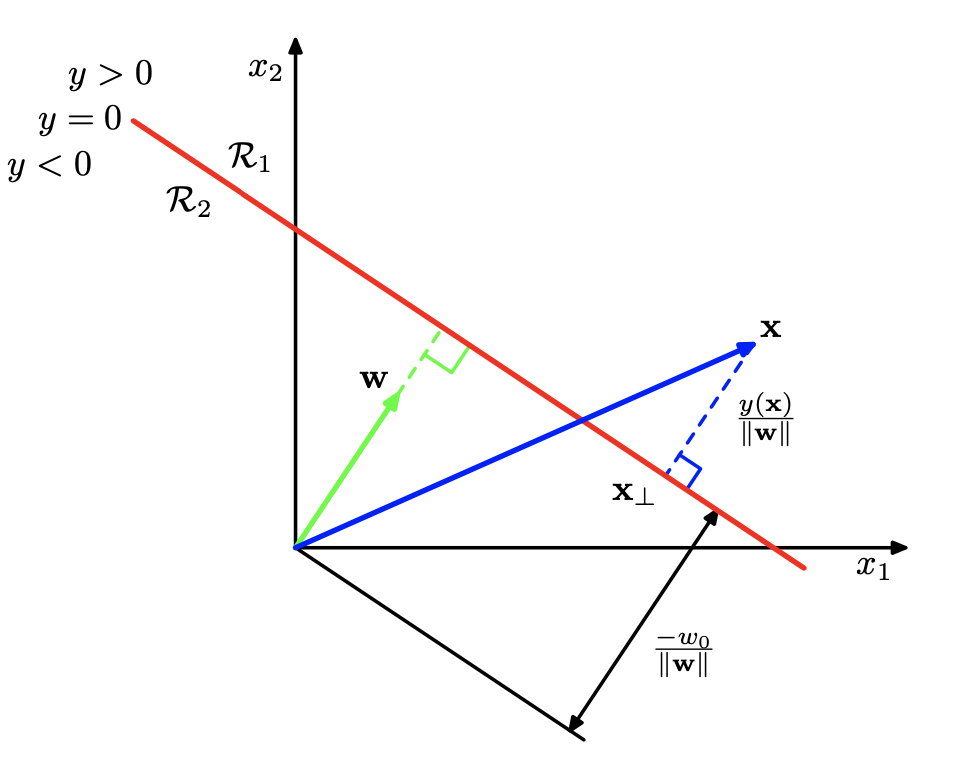
\includegraphics[width=0.40\textwidth]{img/discriminant.png}
    \caption{Illustration of the geometry of a linear discriminant function in two dimensions. The decision surface, shown in red, is perpendicular to $\boldsymbol{w}$, and its displacement from the origin is controlled by the bias parameter $w_0$. Also, the signed orthogonal distance of a general point $\boldsymbol{x}$ from the decision surface is given by $y(\boldsymbol{x}) / \norm{\boldsymbol{w}}$.}
\end{figure}
As with the linear regression models, it is sometimes convenient to use a more compact notation in which we introduce an additionally dummy 'input' value $x_0 = 1$ and then define $\Tilde{\boldsymbol{w}} = (w_0, \boldsymbol{w})$ and $\Tilde{\boldsymbol{x}} = (x_0, \boldsymbol{x})$ so that
\begin{equation*}
    y(\boldsymbol{x}) = \Tilde{\boldsymbol{w}}^\intercal\Tilde{\boldsymbol{x}}
\end{equation*}
In this case, the decision surface are $D$-dimensional hyperplanes passing through the origin of the $D + 1$-dimensional expanded input space. 
\newpage
\subsection{Multiple classes}
Now consider the extension of linear discriminants to $K > 2$ classes. We might be tempted to build a $K$-class discriminant by combining a number of two-class discriminant functions. However, this leads to some serious difficulties.\\
Consider the use of $K -1$ classifiers each of which solves a two-class problem of separating points in a particular class $\mathcal{C}_k$ from points not in that class. This is known as a \textit{one-versus-the-rest} classifier.\medskip

\begin{figure}[h]
    \centering
    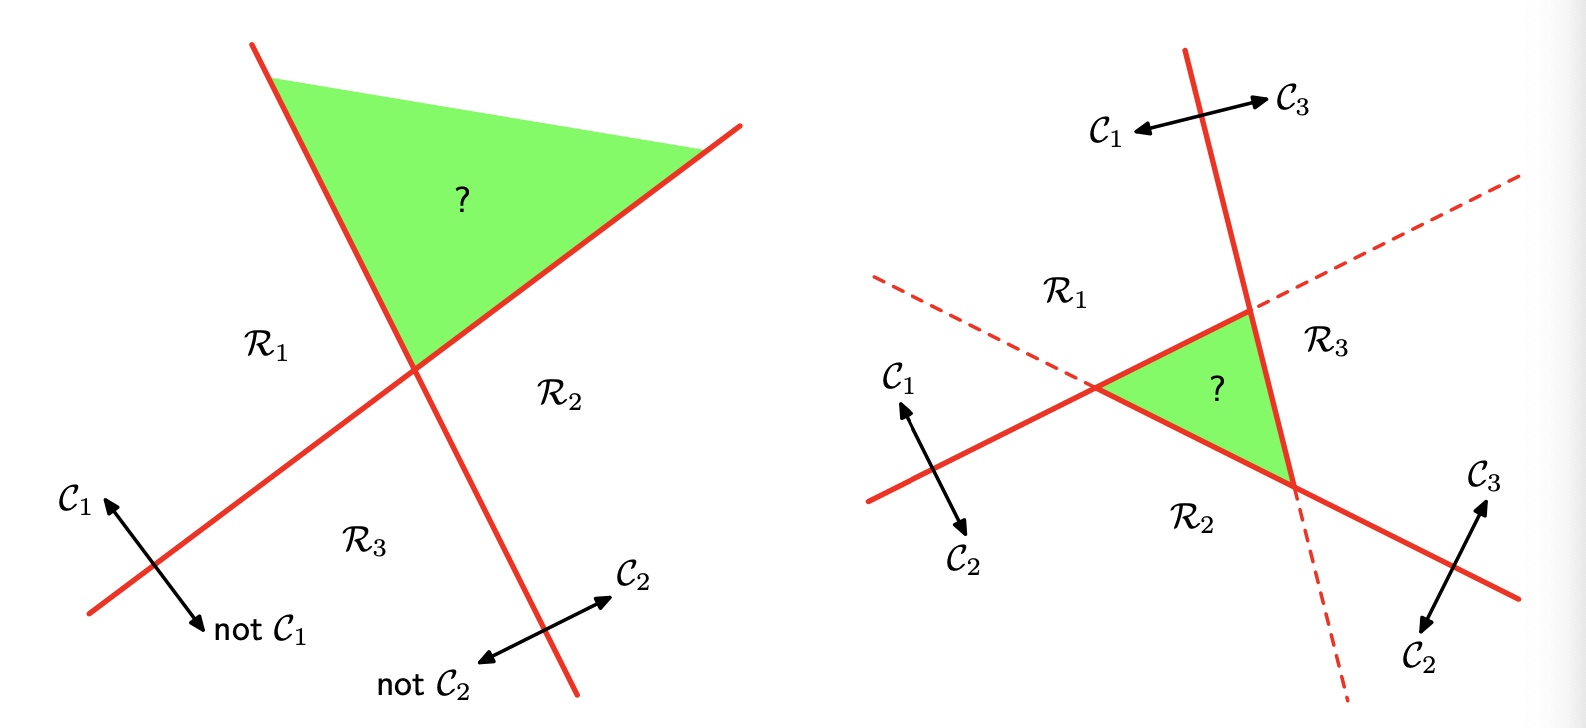
\includegraphics[width=0.50\textwidth]{img/multiclass.png}
    \caption{Attempting to construct a $K$ class discriminant from a set of two class discriminants leads to ambiguous regions, shown in green. On the left is an example involving the use of two discriminants designed to distinguish points in class $\mathcal{C}_k$ from points not in class $\mathcal{C}_k$. On the right is an example involving three discriminant functions each of which is used to separate a pair of classes $\mathcal{C}_k$ and $\mathcal{C}_j$.}
\end{figure}
The left hand example in Figure 6.2 shows an example involving three classes where this approach leads to regions of input space that are ambiguously classified.\medskip

An alternative is to introduce $K(K - 1) / 2$ binary discriminant functions, one for every possible pair of classes. This is known as a \textit{one-versus-one} classifier. Each point is then classified according to a majority vote amongst the discriminant functions. However, this too runs into the problem of ambiguous regions, as illustrated in the right-hand diagram of Figure 6.2.
\newpage
We can avoid these difficulties by considering a single $K$-class discriminant comprising $K$ linear functions of the form
\begin{equation*}
    y_k(\boldsymbol{x}) = \boldsymbol{w_k^\intercal x} + w_{k0}
\end{equation*}
and then assigning a point $\boldsymbol{x}$ to class $\mathcal{C}_k$ if $y_k(\boldsymbol{x}) > y_j(\boldsymbol{x})$ for all $j \neq k$. The decision boundary between class $\mathcal{C}_k$ and class $\mathcal{C}_j$ is therefore given by $y_k(\boldsymbol{x}) = y_j(\boldsymbol{x})$ and hence corresponds to a $(D-1)$-dimensional hyperplane defined by
\begin{equation*}
    (\boldsymbol{w}_k - \boldsymbol{w}_j)^\intercal\boldsymbol{x} + (w_{k0} - w_{j0}) = 0
\end{equation*}
This has the same form as the decision boundary for the two-class case and so analogous geometrical properties apply.

\subsection{Fisher’s linear discriminant}
One way to view a linear classification model is in terms of dimensionality reduction. Consider first the case of two classes, and suppose we take the $D$-dimensional input vector $\boldsymbol{x}$ and project it down to one dimension using
\begin{equation*}
    y = \boldsymbol{w^\intercal x}
\end{equation*}
If we place a threshold on $y$ and classify $y \geq -w_0$ as class $\mathcal{C}_1$, and otherwise class $\mathcal{C}_2$, then we obtain our standard linear classifier.\\
In general, the projection onto one dimension leads to a considerable loss of information, and classes that are well separated in the original $D$-dimensional space may become strongly overlapping in one dimension. However, by adjusting the components of the weight vector $\boldsymbol{w}$, we can select a projection that maximizes the class separation. To begin with, consider a two-class problem in which there are $N_1$ points of $\mathcal{C}_1$ and $N_2$ points of class $\mathcal{C}_2$, so that the mean vectors of the two classes are given by
\begin{equation*}
    \boldsymbol{m}_1 = \frac{1}{N_1}\sum\limits_{n \in \mathcal{C}_1} \boldsymbol{x}_n
    \hspace{20pt}
    \boldsymbol{m}_2 = \frac{1}{N_2}\sum\limits_{n \in \mathcal{C}_2} \boldsymbol{x}_n
\end{equation*}
The simplest measure of the separation of the classes when projected onto $\boldsymbol{w}$, is the separation of the projected class means. This suggests that we might choose $\boldsymbol{w}$ so as to maximize
\begin{equation*}
    m_2 - m_1 = \boldsymbol{w}^\intercal(\boldsymbol{m}_2 - \boldsymbol{m}_1)
\end{equation*}
where 
\begin{equation*}
    m_k = \boldsymbol{w}^\intercal\boldsymbol{m}_k
\end{equation*}
is the mean of the projected data from class $\mathcal{C}_k$. However, this expression can be arbitrarily large simply by increasing the magnitude of $\boldsymbol{w}$. To solve this problem we could constrain $\boldsymbol{w}$ to have unit length, so that $\sum_i w_i^2 = 1$. Using a Lagrange multiplier to perform the constrained maximization, we then find that $\boldsymbol{w} \propto (\boldsymbol{m}_2 - \boldsymbol{m}_1)$. \\
There is still a problem with this approach, however, as illustrated in Figure 6.3. This shows two classes that are well separated in the original two- dimensional space $(x_1, x_2)$ but that have considerable overlap when projected onto the line joining their means. This difficulty arises from the strongly non-diagonal covariances of the class distributions. The idea proposed by Fisher is to maximize a function that will give a large separation between the projected class means while also giving a small variance within each class, thereby minimizing the class overlap.
\newpage
\begin{figure}[h]
    \centering
    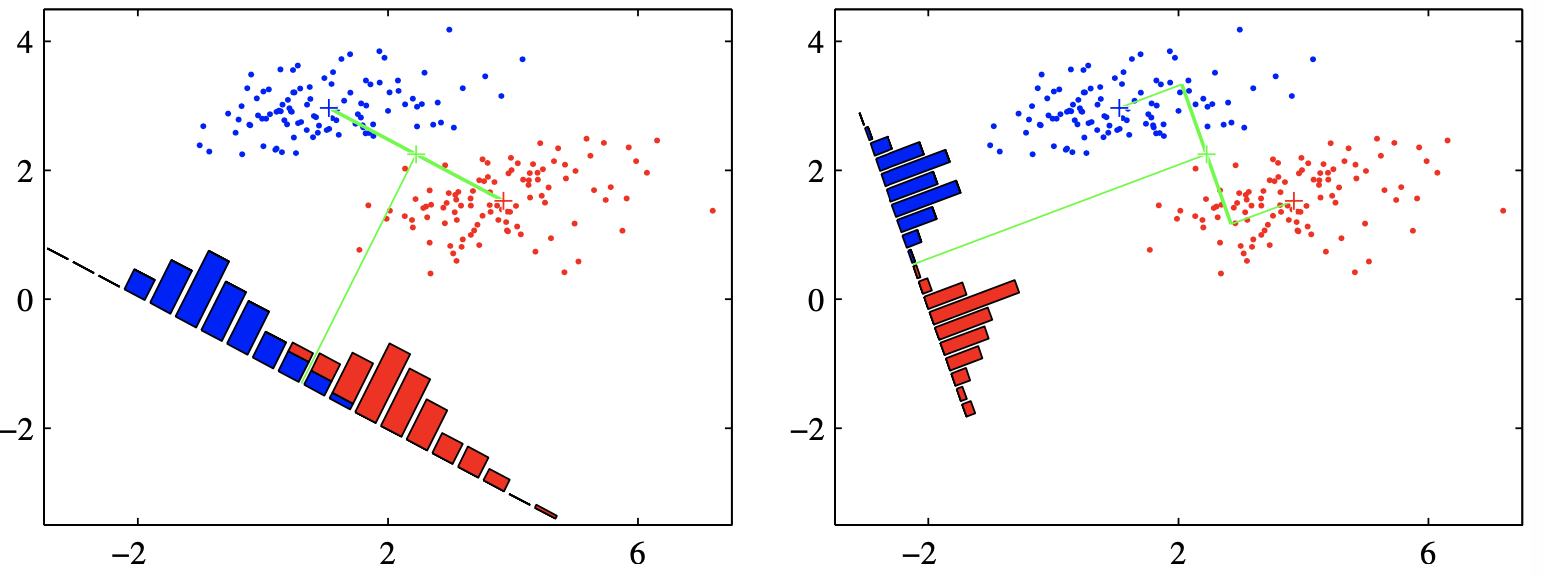
\includegraphics[width=0.70\textwidth]{img/fisher.png}
    \caption{The left plot shows samples from two classes (depicted in red and blue) along with the histograms resulting from projection onto the line joining the class means. Note that there is considerable class overlap in the projected space. The right plot shows the corresponding projection based on the Fisher linear discriminant, showing the greatly improved class separation.}
\end{figure}
\end{document}